\documentclass[11pt,a4paper]{article}

\usepackage[T1]{fontenc}
\usepackage[utf8]{inputenc}
\usepackage{lmodern}
\usepackage[english]{babel}
\usepackage[a4paper,margin=2.5cm]{geometry}
\usepackage{microtype}
\usepackage{amsmath,amssymb}
\usepackage{booktabs,tabularx,multirow,makecell}
\usepackage{graphicx}
\usepackage[font=small,labelfont=bf,skip=4pt]{caption}
\usepackage[round,authoryear]{natbib}
\usepackage{xcolor}
\usepackage[colorlinks=true,linkcolor={blue!50!black},citecolor={blue!50!black},urlcolor={blue!50!black}]{hyperref}
\usepackage{enumitem}
\usepackage{xurl}
\usepackage[section]{placeins}
\setlist{itemsep=2pt,topsep=4pt}
\graphicspath{{../figures/en/}}
\setlength{\parskip}{3pt}
\renewcommand{\arraystretch}{1.12}
\renewcommand{\topfraction}{0.85}
\renewcommand{\bottomfraction}{0.6}
\renewcommand{\textfraction}{0.12}
\renewcommand{\floatpagefraction}{0.8}
\setcounter{topnumber}{3}
\setcounter{totalnumber}{4}

\hypersetup{pdftitle={The S\&P 500 Variance Risk Premium},pdfauthor={Borja Izquierdo Piñero},pdfkeywords={VRP, variance risk premium, gradient boosting, purged cross-validation}}
\newcommand{\repourl}{\url{https://github.com/borja-izquierdo/vrp-sp500-options}}
\newcommand{\E}{\mathbb{E}}

\title{\textbf{The S\&P~500 Variance Risk Premium:\\
Gradient-Boosting Forecasts and the Economic Value of the Signal}\\[4pt]
\large Revised and extended version of a Master's thesis}
\author{Borja Izquierdo Piñero}
\date{October 2026}

\begin{document}
\maketitle

\begin{abstract}
\noindent
This paper asks whether a gradient-boosting forecast of the S\&P~500 variance risk premium (VRP) improves a delta-hedged short-volatility strategy, net of costs and out of sample. Using monthly SPX options from 2018 to 2025, the premium is persistent: implied volatility exceeded subsequently realised volatility on 87.4\% of sessions. An XGBoost model with 22 predictors and purged cross-validation lowers the mean squared error by 6\% relative to the historical mean, but the improvement is not significant under the Diebold--Mariano test. At the trading layer the signal adds no value. Every out-of-sample forecast is positive, so the model-driven strategy coincides with unconditional selling, and the forecast does not rank trade outcomes. The advantage over a naive rule reported in the original thesis does not come from the model; the comparison was not like-for-like. The economic outcome depends mainly on hedge calibration and on how collateral is treated. With interest-bearing collateral, sales at the bid and the original hedge band, systematic selling earns a Sharpe ratio of 0.23, but that band was chosen in sample and its optimum is not stable out of sample. A synthetic variance swap confirms these conclusions without any execution assumptions and puts the February 2018 loss at about twenty months of average premium. No difference between strategies is statistically significant.

\medskip
\noindent\textbf{Keywords:} variance risk premium, implied volatility, gradient boosting, purged cross-validation, delta hedging, variance swaps.\\
\textbf{JEL classification:} C53, G13, G17.
\end{abstract}

\vspace{-2pt}
\noindent\fcolorbox{gray!50}{gray!6}{\parbox{\dimexpr\linewidth-2\fboxsep-2\fboxrule}{\small
\textbf{About this version.} This document revises the Master's thesis \textit{Arbitraje estadístico de volatilidad: modelado del Variance Risk Premium mediante Machine Learning} (Statistical volatility arbitrage: modelling the variance risk premium with machine learning), MSc in Financial Planning and Advice (Máster en Asesoramiento y Planificación Financiera), Universidad Rey Juan Carlos, July 2026. It corrects the interpretation of the comparison between the forecast-driven strategy and the systematic rule (Section~\ref{sec:correction}) and adds nested validation, naive benchmarks, statistical tests, execution costs, collateral interest and an analysis with synthetic variance swaps (Sections~\ref{sec:forecast} to \ref{sec:inference}). Code and results are reproducible at \repourl.}}

\section{Introduction}\label{sec:intro}

The volatility implied by index option prices tends to exceed the volatility the index subsequently realises. This gap, the variance risk premium (VRP), is one of the best-documented regularities in derivatives markets \citep{carrwu2009}, and it rewards those who sell volatility. Harvesting it, however, carries a highly asymmetric risk profile: small, frequent gains against rare but very large losses. On 5 February 2018 the VIX went from 18.44 to 37.32 in a single session, and inverse VIX exchange-traded products lost about 97\% of their value before the next open \citep{augustin2021}. On 21 February Credit Suisse announced the early redemption of XIV at USD~5.99 per note \citep{varadarajan2023}.

The question of this paper is whether a machine-learning forecast of the premium allows it to be sold more efficiently than a mechanical rule; that is, whether it improves the risk--return profile of a delta-hedged short-volatility strategy, net of costs and out of sample. To answer it I build a complete system: download and cleaning of SPX option chains, 22 predictors, XGBoost and LightGBM models with a Huber loss and purged cross-validation, and an event-driven backtest engine that sells SPX straddles and delta-hedges them with commissions and slippage.

The contributions are four. First, the system is reproducible end to end with data any researcher can purchase. Second, forecast accuracy is assessed against naive benchmarks with the \citet{dieboldmariano1995} test, not only in absolute terms. Third, forecast quality is separated from economic value: I measure whether the forecast ranks trade outcomes, whether its magnitude improves entry or position sizing, and how much of the result comes from costs, collateral and hedging. Finally, the premium is also measured with synthetic variance swaps, which covers the whole period (including 2021, for which no option chains are available) and quantifies the February 2018 loss.

The results are mixed and are reported without defensive hedging:
\begin{itemize}
  \item The premium exists and is persistent: positive on 87.4\% of sessions, with a mean of 4.95 volatility points.
  \item The model forecasts better than the naive benchmarks on average, but not in every period, and the improvement in squared error is not significant.
  \item The signal does not reach the trading layer. Every forecast of the selected model is positive, so the forecast-driven strategy is equivalent to always selling. Its rank correlation with the outcome of each trade is 0.05.
  \item The comparison with the systematic rule in the original thesis was not like-for-like: the rule's trade count included a period before the evaluation window. On a like-for-like basis there is no advantage attributable to the model.
  \item What drives the result is risk management: the width of the hedge band and, to a lesser extent, interest on collateral. None of the differences between strategies is statistically significant with 6.7 years and 64 trades.
\end{itemize}

The rest of the paper is organised as follows. Section~\ref{sec:framework} summarises the conceptual framework. Section~\ref{sec:data} describes the data and Section~\ref{sec:method} the methodology. Section~\ref{sec:results} presents the results, Section~\ref{sec:limitations} discusses limitations and extensions, and Section~\ref{sec:conclusions} concludes.

\section{Conceptual framework}\label{sec:framework}

\subsection{The variance risk premium}

A variance swap is a forward contract on realised variance. At maturity the buyer receives $N_{\text{var}}\,(RV_{t,T}-K^2)$, where $RV_{t,T}$ is the annualised variance of daily returns between $t$ and $T$ and $K^2$ is the agreed strike. Because entry is costless, $K^2$ is the expectation of realised variance under the risk-neutral measure $\mathbb{Q}$, and \citet{carrwu2009} show that it can be replicated with a static portfolio of out-of-the-money options. The variance risk premium is the difference between the risk-neutral and the physical ($\mathbb{P}$) expectation:
\begin{equation}
  \text{VRP}_t = \E^{\mathbb{Q}}_t[RV_{t,T}] - \E^{\mathbb{P}}_t[RV_{t,T}].
\end{equation}
For equity indices this difference is large and positive from the variance seller's point of view \citep{carrwu2009}. It stems from a structural imbalance between the demand for protection, concentrated in out-of-the-money puts, and the supply from those who absorb tail risk. Market makers who take the other side are short gamma and therefore require compensation for the losses they suffer when prices jump \citep{ang2018,israelov2019}.

Model-free implied volatility (MFIV) is the square root of the 30-day variance swap strike. The VIX methodology computes it from the out-of-the-money options of the two expirations around 30 days \citep{cboe2019}:
\begin{equation}\label{eq:mfiv}
  \sigma^2_{\text{MFIV}} = \frac{2}{T}\sum_i \frac{\Delta K_i}{K_i^2}\,e^{rT}\,Q(K_i) - \frac{1}{T}\left(\frac{F}{K_0}-1\right)^2,
\end{equation}
where $Q(K_i)$ is the mid price of the out-of-the-money option with strike $K_i$, $F$ is the index forward level and $K_0$ is the first strike below $F$. The VIX divided by 100 is, by construction, the 30-day MFIV of the S\&P~500, and it is used as such in this paper.

\subsection{Delta-hedged short volatility}

A short straddle (selling a call and a put with the same strike and expiry) starts with delta close to zero and negative gamma. If the position is hedged continuously, its daily P\&L is approximately
\begin{equation}\label{eq:gamma}
  d\Pi_t \approx \tfrac{1}{2}\,\Gamma_t S_t^2\left(\sigma^2_{\text{imp}}-\sigma^2_{\text{real},t}\right)dt,
\end{equation}
with $\Gamma_t<0$ for the short position \citep{sinclair2008}. The seller gains when realised volatility stays below implied and loses otherwise, and the loss grows convexly with the size of the move. Systematic option-selling indices display this profile: from 1986 to 2018 the CBOE PutWrite index had a volatility of 9.9\% against 14.9\% for the S\&P~500, but a skewness of $-2.10$ and a kurtosis of 9.72 \citep{wilshire2019}.

In practice hedging is discrete. Rebalancing often reduces gamma risk but multiplies costs; rebalancing rarely saves costs but leaves the position exposed. The hedge tolerance band is therefore a first-order economic parameter, as Section~\ref{sec:costs} confirms.

\subsection{Machine learning and time-series validation}

Gradient-boosting models approximate the target function with a sum of regression trees fitted sequentially to the pseudo-residuals of the previous ensemble \citep{friedman2001}. XGBoost uses a second-order approximation of the loss and L1 and L2 regularisation of leaf weights \citep{chen2016}; LightGBM grows trees leaf-wise and uses gradient-based sampling \citep{ke2017}. Compared with linear models and the GARCH family \citep{bollerslev1986}, they capture non-linearities and interactions without specifying them in advance, an advantage documented in forecasting problems with many predictors \citep{medeiros2021}.

In financial time series, random cross-validation introduces look-ahead bias. When the target is built with future information, as here with the volatility of the next 21 sessions, training and test labels also overlap. \citet{lopezdeprado2018} proposes purging the training observations whose labels overlap the test block and adding an embargo period.

\section{Data}\label{sec:data}

\begin{table}[!htbp]
\centering
\caption{Data sources}\label{tab:data}
\small
\begin{tabularx}{\linewidth}{@{}>{\raggedright\arraybackslash}p{3.3cm}X>{\raggedright\arraybackslash}p{4.4cm}@{}}
\toprule
Source & Series & Use \\
\midrule
ThetaData (Options Standard plan) & SPX monthly options (third Friday): end-of-day quotes, greeks, implied volatility and open interest & Predictors, position selection and valuation \\
Stooq (yfinance as fallback) & SPX daily open, high, low and close & Realised volatility, hedging, buy \& hold \\
FRED & VIXCLS, DGS3MO, DGS10 & MFIV, rates, curve slope, collateral \\
yfinance & CBOE SKEW index & Tail-risk predictor \\
\bottomrule
\end{tabularx}
\end{table}

The sample runs from 2 January 2018 to 31 December 2025: 2,011 sessions and 96 monthly expirations (Table~\ref{tab:data}). SPX options are used rather than SPY options because they are European-style, cash-settled and form the deepest volatility market, on which the VIX itself is computed \citep{cboe2019}.

The chain is cleaned with five filters: positive volume and open interest of at least 100 contracts; valid quotes ($0<\text{bid}<\text{ask}$); relative spread no greater than 20\% of the mid price; 15 to 45 days to expiry; and moneyness ($K/S$) between 0.85 and 1.15. After cleaning, 341,094 observations remain, about 7--9\% of the raw chain.

The 2021 chains could not be retrieved because of a download failure. For that year the model has the market and realised-volatility predictors but not the option microstructure ones, and the option strategy does not trade. The variance swap analysis (Section~\ref{sec:varswap}) does not depend on options and does cover 2021.

\section{Methodology}\label{sec:method}

\subsection{Target}

The target is the realised 21-session volatility premium:
\begin{equation}\label{eq:target}
  y_t = \sigma_{\text{MFIV},t} - \sigma^{\text{YZ}}_{(t,\,t+21]},
\end{equation}
where $\sigma_{\text{MFIV},t}$ is the VIX divided by 100 and $\sigma^{\text{YZ}}$ is the \citet{yangzhang2000} estimator over the next 21 sessions. This estimator combines the overnight jump, the open-to-close move and the Rogers--Satchell term, and is unbiased in the presence of drift and opening jumps. The premium is expressed in volatility: 0.05 equals 5 volatility points.

\subsection{Predictors}

The 22 predictors (Table~\ref{tab:features}) use only information available at the close of session $t$ and fall into three families: realised volatility over 21-session windows, with the close-to-close, \citet{parkinson1980}, \citet{garmanklass1980} and Yang--Zhang estimators; option-market microstructure, measured on the expiry closest to 30 days; and market and momentum variables.

\begin{table}[!htbp]
\centering
\caption{Predictors}\label{tab:features}
\small
\begin{tabularx}{\linewidth}{@{}lX@{}}
\toprule
Family & Variables \\
\midrule
Realised volatility (21 sessions) & \texttt{rv\_cc}, \texttt{rv\_parkinson}, \texttt{rv\_gk}, \texttt{rv\_yz} \\
Option microstructure & \texttt{atm\_iv}; \texttt{skew\_slope} (IV of the $-0.25$-delta put minus IV of the $0.25$-delta call); \texttt{pcr\_volume}, \texttt{pcr\_oi}; \texttt{iv\_rank}, \texttt{iv\_percentile} (252 sessions) \\
Market and momentum & \texttt{mfiv}, \texttt{vix}, \texttt{vix\_chg}, \texttt{skew}, \texttt{skew\_chg}, \texttt{ust\_3m}, \texttt{ust\_10y}, \texttt{term\_slope}; \texttt{ret\_5d}, \texttt{ret\_10d}, \texttt{ret\_21d}, \texttt{ret\_63d} \\
\bottomrule
\end{tabularx}
\end{table}

\subsection{Models and validation}

XGBoost and LightGBM are compared with a Huber loss \citep{huber1964} with threshold $\delta=0.02$, which is quadratic for small errors and linear for large ones and so limits the influence of extreme episodes such as March 2020. Hyper-parameters are chosen by a random search of 40 combinations on a grid (Appendix~\ref{app:hyper}), with a fixed seed.

Validation is time-ordered with an expanding window and five folds. Between the end of each training block and the start of the test block, $21+5$ sessions are dropped: 21 of purge (the label length) and 5 of embargo. In the original thesis, the hyper-parameter search and the choice between XGBoost and LightGBM were scored on the same folds that were then reported. This revision adds \textbf{nested validation}: for each outer fold, both models run their search on a three-fold purged inner validation inside the training block, and the model and parameters with the lowest inner loss are refitted on the whole block and predict the test block. No decision evaluated on a block uses information from that block.

\subsection{Naive benchmarks and tests of predictive accuracy}

The model is compared with two forecasts without learning, scored on the same folds: the mean of the target in the training block, and the naive premium $\sigma_{\text{MFIV},t}-\sigma^{\text{YZ}}_{(t-21,\,t]}$, which assumes realised volatility stays at its recent level. Equal predictive accuracy is tested with the \citet{dieboldmariano1995} statistic, using a \citet{neweywest1987} long-run variance with 20 lags (because the 21-session labels overlap) and the small-sample correction of \citet{hln1997}.

\subsection{Option strategy}\label{sec:strategy}

The strategy is that of the original thesis. When no position is open and the session's signal exceeds the threshold, it sells an at-the-money straddle on the expiry closest to 30 days. The position is marked daily at chain mid prices and hedged with the index whenever the absolute net delta exceeds the band $b\times$ contracts $\times$ multiplier. Each hedge trade pays 1 basis point of slippage and each option 1 dollar of commission, and the position is settled at expiry at intrinsic value. When an option has no quote, which happens systematically in the last 15 days because of the maturity filter, it is valued with Black--Scholes \citep{blackscholes1973,merton1973} at the last observed implied volatility. Size is one contract on USD~1 million of capital; with the SPX at 2,943 at the start of the window, each leg is about USD~294,000 of notional.

The evaluation window runs from 29 April 2019, the first out-of-sample forecast, to 31 December 2025. On this basis two configurations are defined:
\begin{itemize}
  \item \textbf{Thesis configuration}: entry at mid, no interest on collateral, Sharpe ratio with a fixed 2\% risk-free rate, and band $b=0.50$, chosen in the original thesis for its result on the same sample.
  \item \textbf{Rigorous configuration}: sales at the bid, collateral accruing daily at the three-month Treasury bill yield (DGS3MO), Sharpe computed on returns in excess of that same rate, predictions from the nested validation, and a band chosen in each fold. The band is the one that maximises the Sharpe of unconditional selling on the data before the test block.
\end{itemize}
To measure the value of the forecast's magnitude, not just its sign, five signals are compared: always sell; ML $>0$ (the original rule); ML $>$ median, which sells only when the forecast exceeds the median realised premium of the training block; ML sized, which sells $\min(\max(\hat y_t/m,0),3)$ contracts, with $m$ that same median; and naive $>$ median, which applies the same threshold to the naive premium. All thresholds are set with training-block information only.

\subsection{Synthetic variance swaps}\label{sec:method_vs}

To measure the premium independently of the option engine, I simulate the sale of 21-session variance swaps struck at $K=\text{VIX}_t$ (in volatility points). The P\&L per unit of vega notional is
\begin{equation}\label{eq:vswap}
  \pi_t = \frac{K_t^2 - RV_{(t,\,t+21]}}{2K_t},
  \qquad RV_{(t,\,t+21]} = \frac{252}{21}\sum_{i=1}^{21} r_{t+i}^2 \times 10^4,
\end{equation}
with $r$ the daily SPX log returns. A swap with USD~100,000 of vega notional gains or loses USD~100,000 per point of $\pi_t$. The strategy sells one swap every 21 sessions, without overlap, and statistics are averaged over the 21 possible entry calendars. As a robustness check, realised volatility is capped at 2.5 times the strike, as is customary. The analysis ignores that swaps trade somewhat above VIX squared because of convexity and jumps.

\subsection{Inference on strategies}

Confidence intervals for the Sharpe ratio and for Sharpe differences between strategies are obtained with the stationary bootstrap of \citet{politisromano1994}, with a mean block length of 21 sessions and 10,000 resamples. Both series in each comparison are resampled with the same blocks, in the spirit of \citet{ledoitwolf2008}.

\section{Results}\label{sec:results}

\subsection{The premium: stylised facts}

Figure~\ref{fig:vrp} shows implied volatility and the volatility realised over the next 21 sessions. The premium of Equation~\eqref{eq:target} is positive on 87.4\% of sessions, with a mean of 0.0495 and a standard deviation of 0.0724. Its distribution has a pronounced left tail: the premium turns sharply negative when realised volatility accelerates faster than implied, as in January--February 2018 or February--March 2020, with a minimum of $-0.486$.

\begin{figure}[!htbp]
\centering
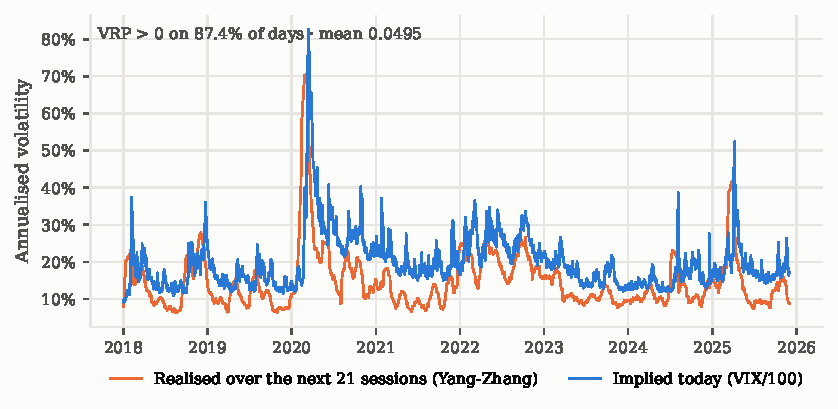
\includegraphics[width=\linewidth]{fig01_vrp_series.pdf}
\caption{Implied volatility (VIX/100) and volatility realised over the next 21 sessions (Yang--Zhang), 2018--2025.}\label{fig:vrp}
\end{figure}

Table~\ref{tab:vs_year} and Figure~\ref{fig:vs_year} present the same premium as a variance swap sold every session. The crisis years (2018 and 2020) have a negative mean result, and 2021 is the best year in the sample: the short swap earned 5.4 volatility points on average and was profitable on 95\% of days. That the option strategy cannot trade in 2021 for lack of data works against it.

\begin{table}[!htbp]
\centering
\caption{Short 21-session variance swap, daily entry (volatility points per unit of vega notional)}\label{tab:vs_year}
\small
\begin{tabular}{@{}lrrrrr@{}}
\toprule
Year & Mean $K$ & Mean $\sqrt{RV}$ & Mean P\&L & \% positive days & Worst day \\
\midrule
2018 & 16.6 & 15.9 & $-1.0$ & 61 & $-25.1$ \\
2019 & 15.4 & 11.2 & 3.1 & 84 & $-15.1$ \\
2020 & 29.3 & 27.1 & $-7.3$ & 77 & $-252.2$ \\
2021 & 19.7 & 12.8 & 5.4 & 95 & $-2.2$ \\
2022 & 25.6 & 23.7 & 1.3 & 65 & $-19.8$ \\
2023 & 16.9 & 12.6 & 3.7 & 100 & 0.1 \\
2024 & 15.6 & 12.4 & 2.4 & 81 & $-11.2$ \\
2025 & 19.3 & 16.0 & 0.8 & 83 & $-59.3$ \\
\bottomrule
\end{tabular}
\end{table}

\begin{figure}[!htbp]
\centering
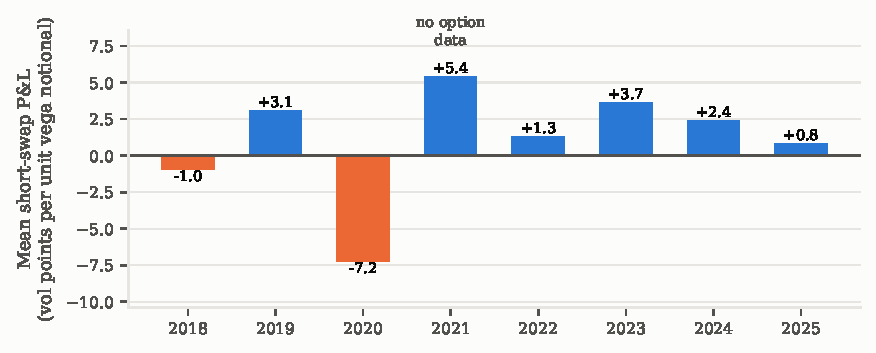
\includegraphics[width=\linewidth]{fig02_varswap_by_year.pdf}
\caption{Mean annual result of a short 21-session variance swap with daily entry. 2021, the year without option chains, is the most favourable for the seller.}\label{fig:vs_year}
\end{figure}

\subsection{Forecast accuracy}\label{sec:forecast}

Table~\ref{tab:forecast} reports the out-of-sample metrics. XGBoost, the model selected in the original thesis, achieves a mean RMSE of 0.0662, 6\% below the training mean (0.0704) and 14\% below the naive premium (0.0766). The improvement is not uniform: the model loses to the training mean in folds 3 and 5 (Figure~\ref{fig:folds}). Under nested validation, which selects LightGBM in the first fold, the mean RMSE rises to 0.0675 and the correlation falls from 0.21 to 0.16. Part of the original advantage therefore came from choosing hyper-parameters on the same evaluation data.

\begin{table}[!htbp]
\centering
\caption{Out-of-sample forecast accuracy: RMSE by fold and means}\label{tab:forecast}
\footnotesize\setlength{\tabcolsep}{4.2pt}
\begin{tabular}{@{}lccccc|cccc@{}}
\toprule
& \multicolumn{5}{c|}{RMSE by fold} & \multicolumn{4}{c}{Mean across folds} \\
Forecast & 1 & 2 & 3 & 4 & 5 & RMSE & MAE & Corr. & Dir. acc. \\
\midrule
XGBoost (thesis) & 0.1289 & 0.0437 & 0.0510 & 0.0356 & 0.0718 & 0.0662 & 0.0426 & 0.212 & 0.905 \\
Nested & 0.1329 & 0.0468 & 0.0506 & 0.0359 & 0.0716 & 0.0675 & 0.0473 & 0.156 & 0.898 \\
Training mean & 0.1295 & 0.0680 & 0.0463 & 0.0386 & 0.0698 & 0.0704 & 0.0491 & -- & 0.905 \\
Naive & 0.1581 & 0.0490 & 0.0539 & 0.0371 & 0.0848 & 0.0766 & 0.0512 & 0.110 & 0.848 \\
\bottomrule
\end{tabular}
\par\smallskip\raggedright\footnotesize Test folds: Apr 2019--Aug 2020, Aug 2020--Dec 2021, Dec 2021--Apr 2023, Apr 2023--Jul 2024 and Aug 2024--Dec 2025.
\end{table}

\begin{figure}[!htbp]
\centering
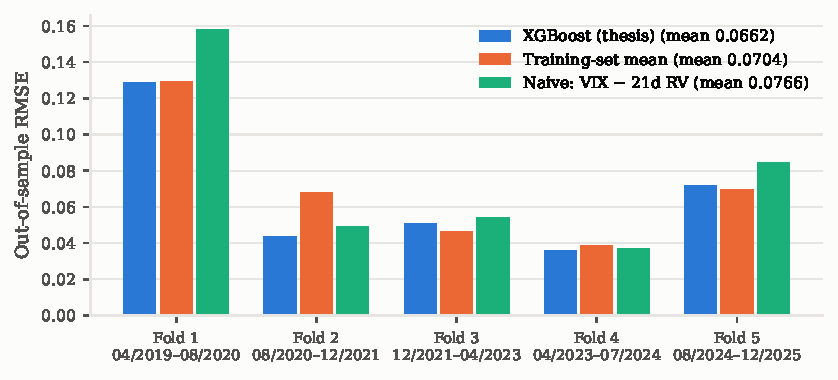
\includegraphics[width=\linewidth]{fig03_forecast_folds.pdf}
\caption{Out-of-sample RMSE by purged validation fold: XGBoost against the training mean and the naive premium.}\label{fig:folds}
\end{figure}

The 90.5\% directional accuracy highlighted in the original thesis carries no information. It equals that of a constant positive forecast, because the premium was positive on 90\% of test days, and Figure~\ref{fig:pred} shows why: the XGBoost forecast ranges from 0.021 to 0.181 and is not negative in any of the 1,659 sessions. The Huber loss and the predominance of positive premia in training lead the model to forecast the typical level of the premium and not to anticipate its drops.

\begin{figure}[!htbp]
\centering
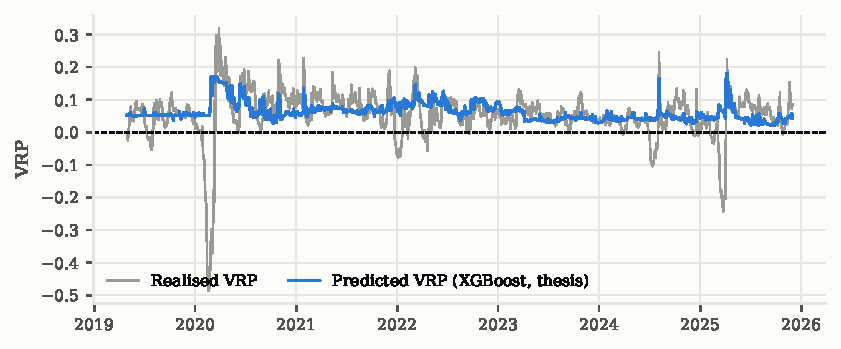
\includegraphics[width=\linewidth]{fig04_prediction_vs_target.pdf}
\caption{Premium forecast by XGBoost (thesis) and realised premium. The forecast never crosses zero.}\label{fig:pred}
\end{figure}

Table~\ref{tab:dm} tests the difference formally. In squared error, the improvement of XGBoost over the training mean is not significant ($p=0.27$); in absolute error it is ($p=0.009$), which indicates that the model does better on normal days without improving on extreme days, which dominate squared error. Against the naive premium the evidence is weak ($p$ between 0.03 and 0.06). Under nested validation no improvement is significant at 5\%.

\begin{table}[!htbp]
\centering
\caption{Diebold--Mariano test (H$_1$: the model is more accurate). HLN-corrected statistic and one-sided $p$-value; $n=1{,}659$}\label{tab:dm}
\small
\begin{tabular}{@{}llcccc@{}}
\toprule
& & \multicolumn{2}{c}{Squared error} & \multicolumn{2}{c}{Absolute error} \\
Model & Benchmark & DM & $p$ & DM & $p$ \\
\midrule
XGBoost (thesis) & Training mean & $-0.61$ & 0.272 & $-2.37$ & 0.009 \\
XGBoost (thesis) & Naive & $-1.52$ & 0.064 & $-1.91$ & 0.028 \\
Nested & Training mean & $-0.87$ & 0.192 & $-1.05$ & 0.147 \\
Nested & Naive & $-1.63$ & 0.052 & $-1.12$ & 0.132 \\
\bottomrule
\end{tabular}
\end{table}

Feature importance of the thesis model, refitted on the full sample, is concentrated in the level of implied volatility (\texttt{mfiv} 0.126 and \texttt{vix} 0.123), followed by the three-month and ten-year yields (0.079 and 0.053) and at-the-money implied volatility (0.052). This is economically coherent, since the starting level of implied volatility is the main driver of the premium, but it is an in-sample measure and should not be read as causal evidence.

\subsection{From forecast to trade}

That the model forecasts something does not mean the information is useful for trading. To measure this directly, Figure~\ref{fig:trades} relates, for the 64 trades of unconditional selling, the outcome of each straddle to the forecast premium at entry. The Spearman rank correlation is 0.05 ($p=0.33$ in a permutation test) with the thesis forecasts and $-0.04$ with the nested ones. The naive premium does not rank trades either (0.05), whereas the VIX level at entry does so weakly (0.21; $p=0.05$). The distribution of outcomes illustrates the strategy's risk: the mean result is USD~929 and 59\% of trades are winners, but the worst one, opened on 21 February 2020, loses USD~43,100, the equivalent of 46 average trades.

\begin{figure}[!htbp]
\centering
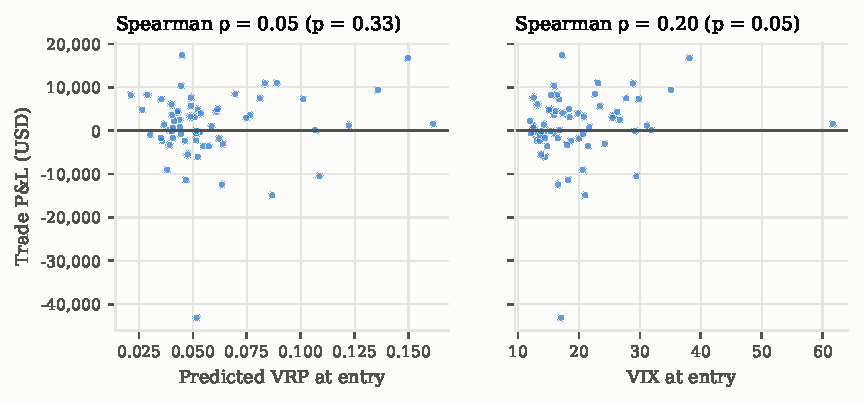
\includegraphics[width=\linewidth]{fig05_trade_level.pdf}
\caption{Outcome of each of the 64 trades of unconditional selling against the forecast premium and the VIX at entry.}\label{fig:trades}
\end{figure}

\subsection{The comparison with the systematic rule, revisited}\label{sec:correction}

The original thesis concluded that the model added tangible value over a systematic rule based on the naive premium: a cumulative return of 5.95\% against 3.89\%, with lower risk and greater selectivity (64 trades against 76). Table~\ref{tab:correction} reproduces those results exactly and shows why the conclusion does not hold.

\begin{table}[!htbp]
\centering
\caption{The original comparison, revisited (thesis configuration, 29/04/2019--31/12/2025)}\label{tab:correction}
\small
\begin{tabular}{@{}lcccc@{}}
\toprule
& ML (thesis) & Always sell & \makecell{Systematic\\(from 2018)} & \makecell{Systematic\\(from window start)} \\
\midrule
Total return (\%) & 5.95 & 5.95 & 3.89 & 3.92 \\
CAGR (\%) & 0.87 & 0.87 & 0.57 & 0.58 \\
Annual volatility (\%) & 2.49 & 2.49 & 2.54 & 2.46 \\
Sharpe (rf 2\%) & $-0.44$ & $-0.44$ & $-0.55$ & $-0.57$ \\
Max drawdown (\%) & $-5.23$ & $-5.23$ & $-6.13$ & $-5.93$ \\
Daily CVaR 95\% (\%) & 0.45 & 0.45 & 0.46 & 0.44 \\
Trades in window & 64 & 64 & 62 (76) & 63 \\
\bottomrule
\end{tabular}
\par\smallskip\raggedright\footnotesize In brackets, the figure in the original thesis, which included 14 trades opened between January 2018 and April 2019.
\end{table}

The comparison was not like-for-like for two reasons. First, because every forecast is positive and the entry threshold is zero, the forecast-driven strategy sells whenever it is flat: its simulation matches that of always selling session by session (first and second columns), and the model takes part in no decision. Second, the systematic strategy was simulated from January 2018, because its signal is available from the start, and its equity curve was then cut to the evaluation window; the trade count, however, was not. Within the window the systematic rule opens 62 trades, not 76, and it is the one that occasionally abstains, because its signal is negative on 6.4\% of days. The return difference comes from those abstentions and from the rule entering the window with a position already open; started on the same day as the forecast-driven strategy, its result barely changes (3.92\%). Figure~\ref{fig:correction} shows the three curves.

\begin{figure}[!htbp]
\centering
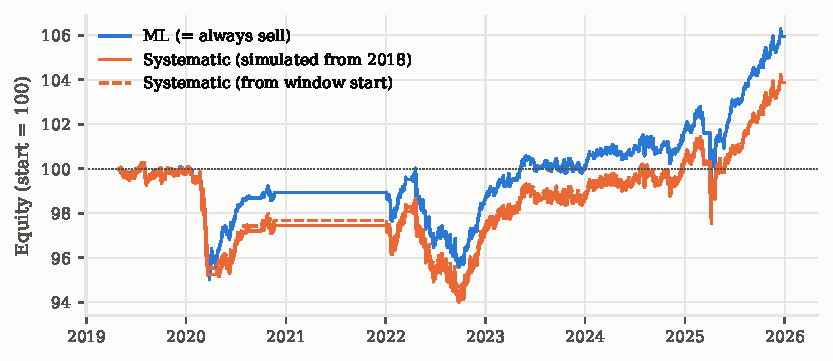
\includegraphics[width=\linewidth]{fig06_corrected_comparison.pdf}
\caption{Equity of the forecast-driven strategy, identical to always selling, and of the systematic rule, simulated from 2018 or from the start of the evaluation window.}\label{fig:correction}
\end{figure}

The correct conclusion is that, in this configuration, the model adds no value over the systematic rule or over unconditional selling. The original thesis did show that the premium exists and that hedging conditions the outcome; what it did not show is that the forecast improves trading.

\subsection{Costs, collateral and hedging}\label{sec:costs}

The negative Sharpe ratio of the original thesis needs a qualification. In the simulation, the USD~1 million of capital earns no interest, yet the Sharpe ratio subtracts 2\% a year. With a one-contract size, the strategy's return is small relative to that hurdle, and the sign of the Sharpe ratio reflects the convention more than the strategy. Table~\ref{tab:costs} and Figure~\ref{fig:steps} decompose the effect of each assumption on unconditional selling.

\begin{table}[!htbp]
\centering
\caption{Unconditional selling: cumulative effect of each assumption (29/04/2019--31/12/2025)}\label{tab:costs}
\small
\begin{tabular}{@{}lcccc@{}}
\toprule
& \makecell{Thesis\\(mid, rf 2\%)} & \makecell{+ collateral\\at 3M T-bill} & \makecell{+ sell\\at bid} & \makecell{+ nested\\band} \\
\midrule
Total return (\%) & 5.95 & 26.08 & 24.33 & 11.62 \\
CAGR (\%) & 0.87 & 3.54 & 3.32 & 1.66 \\
Annual volatility (\%) & 2.49 & 2.28 & 2.30 & 3.66 \\
Sharpe & $-0.44$ & 0.33 & 0.23 & $-0.29$ \\
Max drawdown (\%) & $-5.23$ & $-4.61$ & $-4.66$ & $-10.45$ \\
\bottomrule
\end{tabular}
\par\smallskip\raggedright\footnotesize From the second column on, the Sharpe ratio is computed on returns in excess of the three-month T-bill (2.8\% on average over the window).
\end{table}

\begin{figure}[!htbp]
\centering
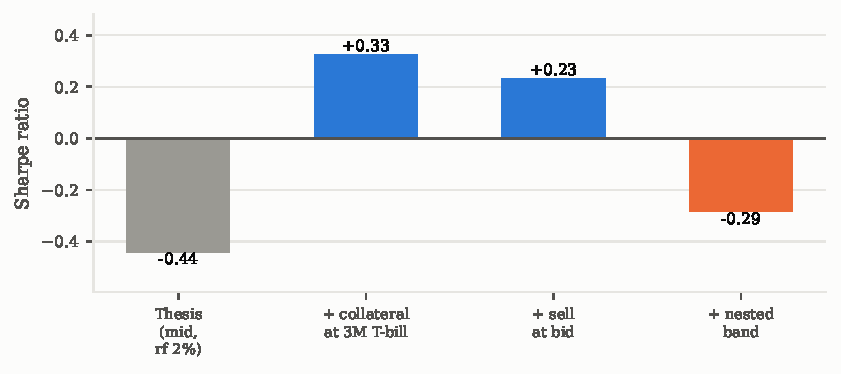
\includegraphics[width=0.85\linewidth]{fig07_sharpe_steps.pdf}
\caption{Sharpe ratio of unconditional selling as each assumption is added.}\label{fig:steps}
\end{figure}

Paying the T-bill rate on collateral, as happens with the margin of a real portfolio, and measuring excess returns over that rate raises the Sharpe ratio from $-0.44$ to 0.33. Selling at the bid rather than at mid costs 1.7 points of cumulative return and lowers the Sharpe ratio to 0.23. With correct accounting, delta-hedged short volatility earns a positive, if small, excess return.

The last step is the most important one. The 0.50 band was chosen in the original thesis as the one that maximised return on the same sample being evaluated (Figure~\ref{fig:band}): a narrow band eats the premium in costs (886 rebalances at 0.05) and no hedging leaves gamma exposed (maximum drawdown of $-15.85$\%). When the band is chosen in each fold using prior data, the choice jumps around with no pattern: unhedged, 1.00, 0.05, 1.00 and 0.50 (Table~\ref{tab:band}). The Sharpe ratio drops to $-0.29$ and the maximum drawdown doubles. The inverted U of Figure~\ref{fig:band} is real in sample, but its peak cannot be identified in advance.

\begin{figure}[!htbp]
\centering
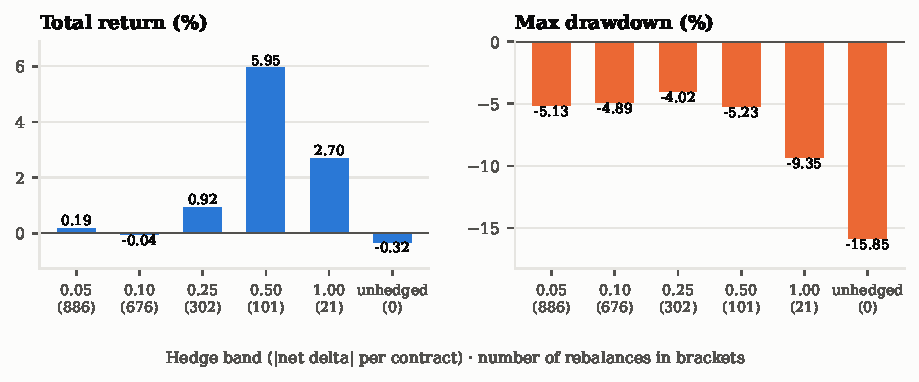
\includegraphics[width=\linewidth]{fig08_hedge_band.pdf}
\caption{Sensitivity of total return and maximum drawdown to the hedge band (thesis configuration, forecast-driven strategy).}\label{fig:band}
\end{figure}

\begin{table}[!htbp]
\centering
\caption{Nested band choice: Sharpe of unconditional selling on the data before each fold}\label{tab:band}
\small
\begin{tabular}{@{}lcccccc|c@{}}
\toprule
Fold (data up to) & 0.05 & 0.10 & 0.25 & 0.50 & 1.00 & Unhedged & Chosen \\
\midrule
1 (20/03/2019) & $-1.54$ & $-1.51$ & $-1.72$ & $-1.91$ & $-1.41$ & $\mathbf{-1.12}$ & Unhedged \\
2 (13/07/2020) & $-0.57$ & $-0.75$ & $-0.86$ & $-0.81$ & $\mathbf{-0.52}$ & $-0.75$ & 1.00 \\
3 (02/11/2021) & $\mathbf{-0.27}$ & $-0.40$ & $-0.48$ & $-0.58$ & $-0.36$ & $-0.57$ & 0.05 \\
4 (28/02/2023) & $-0.59$ & $-0.63$ & $-0.64$ & $-0.39$ & $\mathbf{-0.36}$ & $-0.54$ & 1.00 \\
5 (24/06/2024) & $-0.30$ & $-0.31$ & $-0.35$ & $\mathbf{-0.27}$ & $-0.46$ & $-0.60$ & 0.50 \\
\bottomrule
\end{tabular}
\par\smallskip\raggedright\footnotesize Every training period includes 2018 and, from fold 2 on, March 2020, hence the negative Sharpe ratios.
\end{table}

\subsection{Does the forecast's magnitude help?}\label{sec:magnitude}

The original rule used only the sign of the forecast. Table~\ref{tab:magnitude} evaluates the alternatives that use its magnitude in the rigorous configuration, with the nested band and with the fixed 0.50 band, and Figure~\ref{fig:honest} shows the equity curves.

\begin{table}[!htbp]
\centering
\caption{Using the forecast's magnitude (rigorous configuration, 29/04/2019--31/12/2025)}\label{tab:magnitude}
\small
\begin{tabular}{@{}lcccccc@{}}
\toprule
& \makecell{Always\\sell} & ML $>0$ & \makecell{ML $>$\\median} & \makecell{ML\\sized} & \makecell{Naive $>$\\median} & \makecell{Buy \&\\hold} \\
\midrule
\multicolumn{7}{@{}l}{\textit{Band chosen in each fold (nested)}} \\
Total return (\%) & 11.62 & 11.80 & 20.14 & 15.25 & 16.36 & 132.60 \\
Annual volatility (\%) & 3.66 & 3.65 & 1.65 & 2.61 & 3.25 & 20.23 \\
Sharpe & $-0.29$ & $-0.28$ & 0.00 & $-0.23$ & $-0.13$ & 0.59 \\
Max drawdown (\%) & $-10.45$ & $-10.53$ & $-2.44$ & $-5.95$ & $-10.35$ & $-33.93$ \\
Daily CVaR 95\% (\%) & 0.60 & 0.60 & 0.28 & 0.45 & 0.49 & 3.07 \\
\midrule
\multicolumn{7}{@{}l}{\textit{Band fixed at 0.50}} \\
Total return (\%) & 24.33 & 24.50 & 23.12 & 23.39 & 25.19 & -- \\
Annual volatility (\%) & 2.30 & 2.30 & 1.69 & 2.12 & 1.81 & -- \\
Sharpe & 0.23 & 0.24 & 0.22 & 0.20 & 0.35 & -- \\
Max drawdown (\%) & $-4.66$ & $-4.65$ & $-3.29$ & $-5.26$ & $-4.33$ & -- \\
Daily CVaR 95\% (\%) & 0.40 & 0.40 & 0.28 & 0.38 & 0.30 & -- \\
\midrule
Trades & 64 & 64 & 30 & 64 & 42 & -- \\
\bottomrule
\end{tabular}
\par\smallskip\raggedright\footnotesize ML sized: 0.82 contracts on average. Sharpe is the excess over the three-month T-bill; collateral earns that rate.
\end{table}

With the nested band, trading only when the forecast premium exceeds the historical median halves volatility, cuts the maximum drawdown from $-10.5$\% to $-2.4$\%, and raises the Sharpe ratio from $-0.29$ to 0.00. The result looks attractive at first sight, but it comes mainly from trading less (30 trades against 64) in a configuration where the hedge is badly calibrated: with the band fixed at 0.50, the same rule does not beat unconditional selling (0.22 against 0.23). Proportional sizing does not help in either configuration. The naive rule with the same threshold obtains the best Sharpe with the fixed band (0.35), so if filtering on the level of the premium has any value, it does not require a machine-learning model.

\begin{figure}[!htbp]
\centering
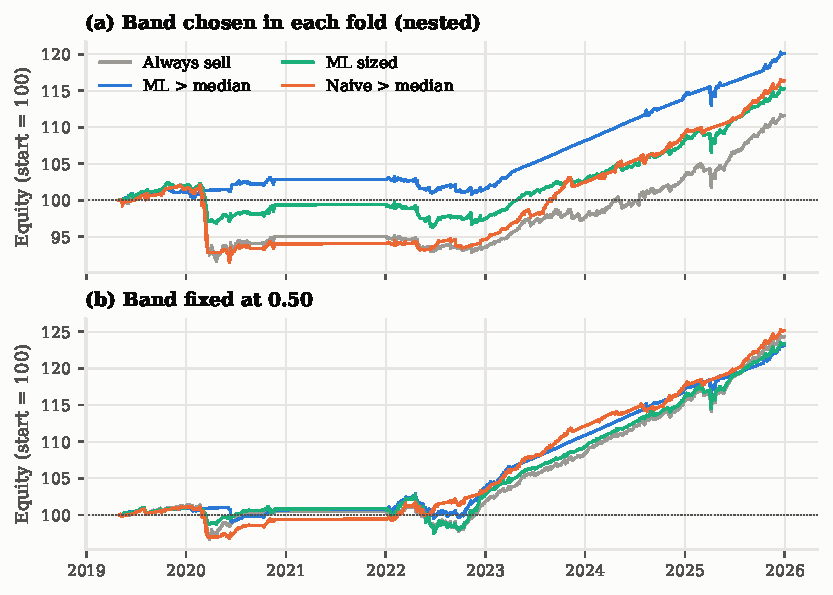
\includegraphics[width=\linewidth]{fig09_honest_equity.pdf}
\caption{Equity of the strategies in the rigorous configuration (sales at the bid, interest-bearing collateral), with the band chosen in each fold and with the band fixed at 0.50.}\label{fig:honest}
\end{figure}

\subsection{The premium in pure form: variance swaps}\label{sec:varswap}

Table~\ref{tab:vs} presents the results of selling monthly variance swaps, averaged over the 21 possible entry calendars, and Figure~\ref{fig:vs} shows the cumulative result and the dispersion across calendars.

\begin{table}[!htbp]
\centering
\caption{Variance swaps sold every 21 sessions (mean over the 21 entry calendars; P\&L in volatility points per unit of vega notional)}\label{tab:vs}
\small
\begin{tabular}{@{}lccccc|cc@{}}
\toprule
& & \multicolumn{4}{c|}{Uncapped} & \multicolumn{2}{c}{Capped at 2.5$\cdot K$} \\
Strategy & \makecell{Months with\\position} & \makecell{Mean\\P\&L} & Sharpe & Skewness & \makecell{Worst\\month} & \makecell{Mean\\P\&L} & Sharpe \\
\midrule
Unconditional, 2018--2025 & 94.8 & 1.06 & 0.28 & $-6.9$ & $-145.8$ & 1.97 & 0.71 \\
Unconditional, window & 79.0 & 1.22 & 0.31 & $-6.8$ & $-145.8$ & 2.32 & 0.81 \\
ML $>0$, window & 78.4 & 1.19 & 0.31 & $-6.7$ & $-145.8$ & 2.29 & 0.80 \\
ML $>$ median, window & 36.0 & 0.31 & 0.50 & $-3.5$ & $-96.1$ & 1.13 & 0.70 \\
Naive $>$ median, window & 38.6 & 1.03 & 0.71 & $-3.9$ & $-77.3$ & 1.32 & 0.81 \\
\bottomrule
\end{tabular}
\par\smallskip\raggedright\footnotesize Mean P\&L includes months without a position (zero result). Annualised Sharpe of monthly results. Window: 29/04/2019--31/12/2025.
\end{table}

\begin{figure}[!htbp]
\centering
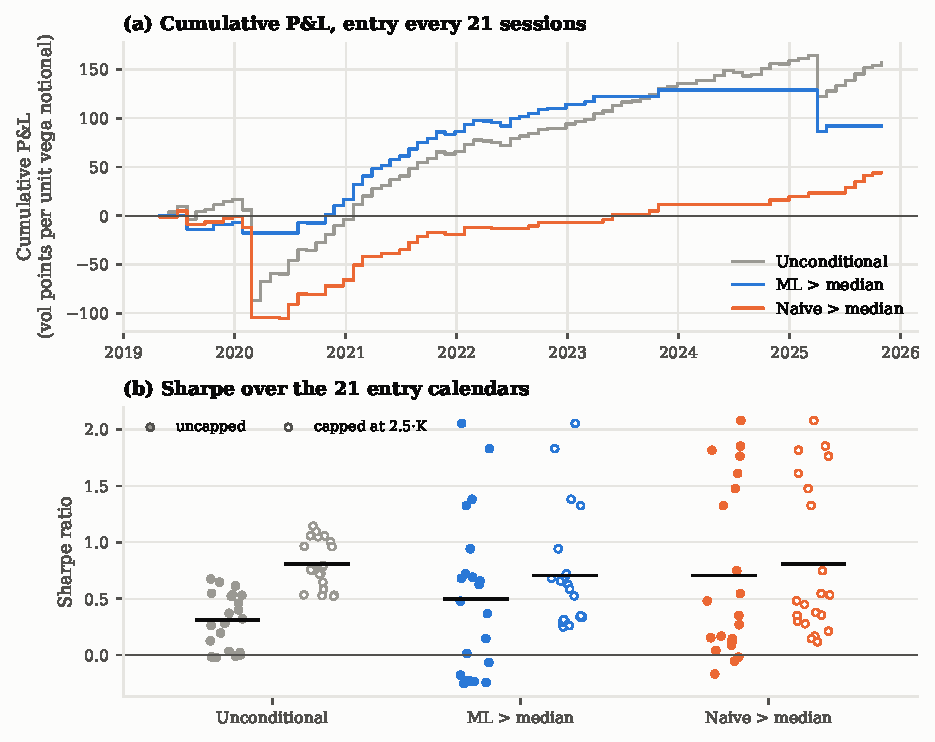
\includegraphics[width=\linewidth]{fig11_varswap.pdf}
\caption{Variance swaps sold every 21 sessions: (a) cumulative result with the first entry calendar; (b) Sharpe ratio of each of the 21 calendars, uncapped and capped at 2.5$\cdot K$ (black lines are the means).}\label{fig:vs}
\end{figure}

Variance swaps confirm the conclusions of the option strategy in a setting that does not depend on execution, hedging or option data. The unconditional premium is positive in 81--83\% of months, but its distribution is very negatively skewed ($-6.9$), and without a cap a single month of 2020 wipes out years of results. Filtering with the model's forecast improves the mean uncapped Sharpe (0.50 against 0.31) at the cost of trading in fewer than half the months, but not the capped one (0.70 against 0.81). The naive rule again does as well or better. Moreover, the dispersion across calendars is very large: depending on the entry date, the Sharpe of the model-filtered strategy ranges from $-0.25$ to 2.05. With about 80 months, the entry date matters as much as the signal.

\subsection{Volmageddon}\label{sec:volmageddon}

Figure~\ref{fig:volm} places the February 2018 episode in this framework. This part is descriptive, because the option backtest starts in 2019. Throughout January 2018 the VIX stayed between 9 and 15, while for swaps sold from 9 January onwards the volatility realised over the next 21 sessions was 23.5 to 26.4 points. A swap sold on 22 January with a strike of 11.0 realised 24.8 points and lost 22.3 points per unit of vega notional, that is, USD~2.2 million per USD~100,000 of vega notional, the equivalent of about 20 months of average premium (1.06 points a month over 2018--2025). The loss did not come from the session of 5 February itself, but from having sold volatility when implied was historically low. Once the jump had occurred, implied exceeded subsequently realised volatility, and swaps sold between 5 and 21 February earned between 3.2 and 12.9 points.

\begin{figure}[!htbp]
\centering
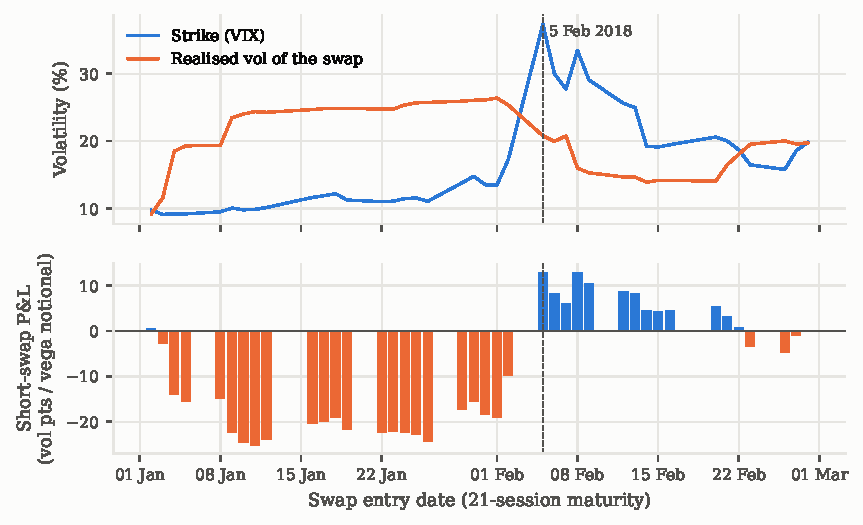
\includegraphics[width=\linewidth]{fig12_volmageddon.pdf}
\caption{Variance swaps sold in January and February 2018: strike (VIX) and volatility realised over the next 21 sessions (top), and result by entry date (bottom). Descriptive analysis; not part of the option backtest.}\label{fig:volm}
\end{figure}

\subsection{Inference}\label{sec:inference}

Figure~\ref{fig:boot} and Table~\ref{tab:boot} summarise the bootstrap confidence intervals. No Sharpe ratio of the volatility strategies differs from zero at 95\% confidence, and no difference against unconditional selling is significant: the largest, ML $>$ median with the nested band, has a 95\% interval of $[-0.45,\,0.95]$. The available sample cannot tell the variants apart, and any ranking in Table~\ref{tab:magnitude} should be read with that caution.

\begin{table}[!htbp]
\centering
\caption{Stationary-bootstrap confidence intervals (rigorous configuration, nested band; 10,000 resamples)}\label{tab:boot}
\footnotesize\setlength{\tabcolsep}{4pt}
\begin{tabular}{@{}lcccc@{}}
\toprule
& Estimate & 95\% CI & 90\% CI & P($\leq 0$) \\
\midrule
Sharpe: always sell & $-0.29$ & $[-0.84,\ 0.49]$ & $[-0.76,\ 0.38]$ & 0.76 \\
Sharpe: ML $>$ median & 0.00 & $[-0.55,\ 0.60]$ & $[-0.46,\ 0.50]$ & 0.49 \\
Sharpe: buy \& hold & 0.59 & $[-0.03,\ 1.35]$ & $[0.07,\ 1.23]$ & 0.03 \\
Diff.: ML $>0$ $-$ always sell & 0.01 & $[-0.02,\ 0.04]$ & $[-0.01,\ 0.03]$ & 0.37 \\
Diff.: ML $>$ median $-$ always sell & 0.29 & $[-0.45,\ 0.95]$ & $[-0.35,\ 0.85]$ & 0.26 \\
Diff.: ML sized $-$ always sell & 0.06 & $[-0.21,\ 0.24]$ & $[-0.16,\ 0.21]$ & 0.36 \\
Diff.: naive $>$ median $-$ always sell & 0.15 & $[-0.18,\ 0.72]$ & $[-0.12,\ 0.61]$ & 0.18 \\
Swap diff.: ML $>$ median $-$ uncond. & 0.09 & $[-1.62,\ 1.45]$ & $[-1.43,\ 1.25]$ & 0.53 \\
\bottomrule
\end{tabular}
\end{table}

\begin{figure}[!htbp]
\centering
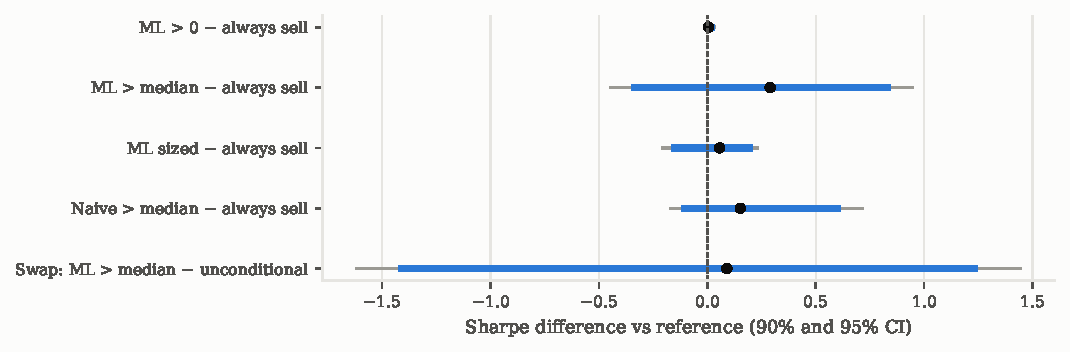
\includegraphics[width=\linewidth]{fig10_bootstrap.pdf}
\caption{Sharpe differences against the reference, with 90\% (thick bar) and 95\% (thin bar) confidence intervals.}\label{fig:boot}
\end{figure}

\section{Limitations and extensions}\label{sec:limitations}

\paragraph{Valuation at the end of the option's life.} The cleaned chain covers 15 to 45 days to expiry, so the last 15 days of each straddle, when gamma peaks, are valued with Black--Scholes at the last implied volatility. This is the most important limitation for tail risk, and the only one that requires new option data: a tracking chain from 0 to 45 days would allow the whole life of the position to be marked at market prices.

\paragraph{The year 2021.} The missing 2021 chains remove the most favourable year for the volatility seller (Table~\ref{tab:vs_year}). The variance swap analysis covers it, but the option strategy does not.

\paragraph{Execution assumptions.} Selling at the bid corrects the entry spread, but hedging is modelled with 1 basis point of slippage and no market impact, settlement uses the close on expiry day rather than the special opening quotation of monthly SPX options, and size is fixed.

\paragraph{Statistical power.} The results rest on a single 6.7-year path, 64 trades and about 80 months, dominated by a bull market. The intervals in Section~\ref{sec:inference} show that this sample cannot distinguish between the variants.

\paragraph{Model selection.} Nested validation removes the selection bias in hyper-parameters and in the band, but the overall design (predictors, horizon, loss, grid) was built with knowledge of the sample.

\paragraph{Extensions.} The most promising lines are: (i) a complete tracking chain and the recovery of 2021; (ii) forecasting the hedged trade's outcome directly, instead of the volatility spread, or recasting the problem as classifying regimes of negative premium; (iii) sizing towards a volatility target using the forecast of risk rather than of the premium; (iv) extending the sample backwards and adding weekly options (SPXW) to increase the number of independent trades; and (v) testing the rules on other assets (VIX, VIX futures, other indices).

\section{Conclusions}\label{sec:conclusions}

The S\&P~500 variance risk premium is persistent and can be harvested: with correct accounting for collateral and sales at the bid, systematic selling of hedged straddles earns a positive excess return with a fraction of the risk of equities. Forecasting the premium with gradient boosting improves on the naive benchmarks on average, but modestly, unstably across periods and not significantly in squared error. That information does not carry over to trading: the model forecasts a positive premium in every session, its forecast does not rank trade outcomes, and rules that use its magnitude do not significantly improve on unconditional selling or on a naive rule.

The economic result is determined by risk management. The hedge band explains more of the variation in outcomes than any signal, and its in-sample optimum cannot be identified in advance. For a volatility seller, the relevant question is not how large the premium will be next month, since its typical level is well known, but when it may turn sharply negative and what it costs to protect against that. That is the problem a next version of this system should address.

\FloatBarrier
\bibliographystyle{plainnat}
\bibliography{../refs}

\clearpage
\appendix
\section{Hyper-parameters}\label{app:hyper}

\begin{table}[!htbp]
\centering
\caption{Search grid (40 random combinations with seed 42) and choice by fold}\label{tab:hyper}
\small
\begin{tabularx}{\linewidth}{@{}lX@{}}
\toprule
Parameter & Values \\
\midrule
Learning rate & 0.01; 0.05; 0.1 \\
Leaves (LightGBM) & 31; 63; 127 \\
Depth (XGBoost) & 3; 5; 7 \\
Row and column subsampling & 0.7; 0.8; 0.9 \\
L1 and L2 regularisation & 0; 0.1; 1; 10 \\
Trees; Huber threshold & 400; $\delta=0.02$ \\
\midrule
Thesis (XGBoost) & rate 0.1; depth 3; subsampling 0.9 and 0.9; L1 1; L2 0.1 \\
Nested, fold 1 & LightGBM: rate 0.1; 63 leaves; 0.8 and 0.8; L1 1; L2 10 \\
Nested, folds 2--5 & XGBoost: depth 3, 5, 7 and 3; otherwise as in the thesis except L2 1 (fold 3) and L1 0.1 (fold 4) \\
\bottomrule
\end{tabularx}
\end{table}

\section{Reproducibility}

The code, organised as a Python package, is available at \repourl. The script \texttt{scripts/run\_pipeline.py} reproduces the results of the original thesis and \texttt{scripts/run\_extensions.py} those of this revision. ThetaData data cannot be redistributed; the repository includes the download script, the out-of-sample forecasts of the original thesis and every results table. Seeds are fixed (42). XGBoost does not produce bit-identical forecasts across platforms: retraining on Linux changes the fold RMSE by up to 0.003 relative to the original run, although every forecast remains positive and the backtest does not change.

\end{document}
